\documentclass[10pt,a4paper]{article}

\usepackage[a4paper,margin=16mm,headheight=15pt]{geometry}
\usepackage{fontspec}
\setmainfont{Tahoma}
\newfontfamily\headingfont{Avenir Next}
\setmonofont[Scale=.83]{Courier New}
\usepackage{microtype}
\usepackage{xcolor}
\definecolor{Navy}{HTML}{102A43}
\definecolor{Blue}{HTML}{2563EB}
\definecolor{Cyan}{HTML}{0891B2}
\definecolor{Teal}{HTML}{0F766E}
\definecolor{Green}{HTML}{15803D}
\definecolor{Amber}{HTML}{B45309}
\definecolor{Red}{HTML}{B42318}
\definecolor{Purple}{HTML}{7C3AED}
\definecolor{Ink}{HTML}{1F2937}
\definecolor{Muted}{HTML}{64748B}
\definecolor{Line}{HTML}{CBD5E1}
\definecolor{Pale}{HTML}{F8FAFC}
\definecolor{PaleBlue}{HTML}{EFF6FF}
\definecolor{PaleTeal}{HTML}{F0FDFA}
\definecolor{PaleGreen}{HTML}{F0FDF4}
\definecolor{PaleAmber}{HTML}{FFFBEB}
\definecolor{PaleRed}{HTML}{FEF2F2}
\definecolor{PalePurple}{HTML}{F5F3FF}

\usepackage{booktabs,longtable,tabularx,array,multirow,colortbl}
\usepackage{enumitem}
\setlist{nosep,leftmargin=1.35em}
\usepackage[most]{tcolorbox}
\usepackage{tikz}
\usetikzlibrary{arrows.meta,calc,fit,matrix,positioning,shapes.geometric}
\usepackage{titlesec}
\usepackage{fancyhdr}
\usepackage{hyperref}
\usepackage{bookmark}
\usepackage{ragged2e}
\usepackage{seqsplit}
\usepackage{lastpage}
\usepackage{needspace}
\newcolumntype{Y}{>{\RaggedRight\arraybackslash}X}
\newcolumntype{L}[1]{>{\RaggedRight\arraybackslash}p{#1}}

\hypersetup{
  colorlinks=true,
  linkcolor=Navy,
  urlcolor=Blue,
  pdftitle={Medicine Search: Rules, Examples, and Current Evaluation},
  pdfauthor={Medicine Search Engineering Team}
}
\titleformat{\section}{\headingfont\fontsize{20}{23}\selectfont\bfseries\color{Navy}}{\thesection}{.65em}{}
\titleformat{\subsection}{\headingfont\large\bfseries\color{Teal}}{\thesubsection}{.55em}{}
\titlespacing*{\section}{0pt}{1.5em}{.65em}
\titlespacing*{\subsection}{0pt}{1.05em}{.4em}
\pagestyle{fancy}
\fancyhf{}
\fancyhead[L]{\headingfont\small Medicine Search Team Handbook}
\fancyhead[R]{\headingfont\small\color{Muted}Latest-source evaluation}
\fancyfoot[L]{\footnotesize\color{Muted}23 August 2026}
\fancyfoot[R]{\footnotesize\color{Muted}\thepage/\pageref*{LastPage}}
\renewcommand{\headrulewidth}{.3pt}
\setlength{\parindent}{0pt}
\setlength{\parskip}{5pt}
\renewcommand{\arraystretch}{1.25}
\setlength{\emergencystretch}{3em}

\newtcolorbox{takeaway}[1][]{enhanced,breakable,colback=PaleBlue,colframe=Blue,
  boxrule=.6pt,arc=2mm,left=3mm,right=3mm,top=2.4mm,bottom=2.4mm,
  fonttitle=\headingfont\bfseries,#1}
\newtcolorbox{safetybox}[1][]{enhanced,breakable,colback=PaleAmber,colframe=Amber,
  boxrule=.6pt,arc=2mm,left=3mm,right=3mm,top=2.4mm,bottom=2.4mm,
  fonttitle=\headingfont\bfseries,#1}
\newtcolorbox{resultbox}[1][]{enhanced,breakable,colback=PaleGreen,colframe=Green,
  boxrule=.6pt,arc=2mm,left=3mm,right=3mm,top=2.4mm,bottom=2.4mm,
  fonttitle=\headingfont\bfseries,#1}
\newtcolorbox{proposedbox}[1][]{enhanced,breakable,colback=PaleRed,colframe=Red,
  boxrule=.6pt,arc=2mm,left=3mm,right=3mm,top=2.4mm,bottom=2.4mm,
  fonttitle=\headingfont\bfseries,#1}

\newcommand{\observed}[1]{\texttt{#1}}
\newcommand{\mapstoex}{\ensuremath{\longrightarrow}}
\newcommand{\yes}{\textcolor{Green}{\headingfont\bfseries PASS}}
\newcommand{\no}{\textcolor{Red}{\headingfont\bfseries NOT ACTIVE}}
\newcommand{\metric}[3]{%
  \begin{minipage}[t]{.29\linewidth}\centering
  {\headingfont\fontsize{21}{23}\selectfont\bfseries\color{#3}#1}\\[-1mm]
  {\small\color{Muted}#2}\end{minipage}}
\newcommand{\caseflow}[3]{%
  \texttt{#1}\enspace\textcolor{Muted}{\mapstoex\ #2\ \mapstoex}\enspace\texttt{#3}}

% AUTO-GENERATED by generate_team_handbook_results.py; do not edit.
% Metrics are bound to preserved artifacts, frozen datasets, and exact core-source hashes.
% Accuracy, safety contracts, and developer regression coverage are deliberately separate.
\newcommand{\OrdinaryCases}{800}
\newcommand{\OrdinaryHitOne}{799}
\newcommand{\OrdinaryHitFive}{800}
\newcommand{\OrdinaryHitTwenty}{800}
\newcommand{\OrdinaryMRR}{0.999375}
\newcommand{\OrdinarySafetyCases}{150}
\newcommand{\OrdinarySafetyPass}{150}
\newcommand{\FairCases}{412}
\newcommand{\FairHitOne}{234}
\newcommand{\FairHitFive}{296}
\newcommand{\FairHitTwenty}{340}
\newcommand{\FairMissTwenty}{72}
\newcommand{\FairMRR}{0.633907}
\newcommand{\FairAFiveHitOne}{234}
\newcommand{\FairAFiveHitFive}{296}
\newcommand{\FairAFiveHitTwenty}{338}
\newcommand{\FairAFiveMRR}{0.633664}
\newcommand{\FairDamerauHitOne}{179}
\newcommand{\FairDamerauHitFive}{251}
\newcommand{\FairDamerauHitTwenty}{299}
\newcommand{\FairDamerauMRR}{0.51581}
\newcommand{\DamerauHitOne}{179}
\newcommand{\DamerauHitFive}{251}
\newcommand{\DamerauHitTwenty}{299}
\newcommand{\DamerauMRR}{0.51581}
\newcommand{\FairJaroHitOne}{149}
\newcommand{\FairJaroHitFive}{256}
\newcommand{\FairJaroHitTwenty}{312}
\newcommand{\FairJaroMRR}{0.478935}
\newcommand{\JaroHitOne}{149}
\newcommand{\JaroHitFive}{256}
\newcommand{\JaroHitTwenty}{312}
\newcommand{\JaroMRR}{0.478935}
\newcommand{\VisualTotalCases}{424}
\newcommand{\VisualContractPass}{424}
\newcommand{\VisualSourceCases}{314}
\newcommand{\VisualSourceHits}{314}
\newcommand{\VisualHitOne}{313}
\newcommand{\VisualHitFive}{314}
\newcommand{\VisualHitTwenty}{314}
\newcommand{\VisualMRR}{0.998408}
\newcommand{\VisualSafetyCases}{100}
\newcommand{\VisualSafetyPass}{100}
\newcommand{\VisualExactLabels}{400}
\newcommand{\VisualExactLabelsFound}{400}
\newcommand{\VisualPrecisionIndicator}{22.1}
\newcommand{\VisualUnexpectedFuzzyIdentities}{1410}
\newcommand{\VisualExtraIdentities}{1410}
\newcommand{\VisualHoldoutCases}{86}
\newcommand{\VisualHoldoutPass}{86}
\newcommand{\VisualCases}{\VisualSourceCases}
\newcommand{\ProductCases}{440}
\newcommand{\ProductPass}{440}
\newcommand{\ProductFirstPass}{435}
\newcommand{\ProductFirstFail}{5}
\newcommand{\ProductUniqueStrengthCases}{240}
\newcommand{\ProductTieCases}{40}
\newcommand{\ProductFormCases}{80}
\newcommand{\ProductAbstentionCases}{80}
\newcommand{\ProductContextCases}{200}
\newcommand{\ProductBaselineHitOne}{197}
\newcommand{\ProductContextBaseline}{197}
\newcommand{\ProductContextHitOne}{200}
\newcommand{\ProductContextRecoveries}{3}
\newcommand{\ProductContextRegressions}{0}
\newcommand{\OcrGeneratedCases}{160}
\newcommand{\OcrGeneratedHitTwenty}{160}
\newcommand{\OcrChallengeCases}{78}
\newcommand{\OcrChallengePass}{78}
\newcommand{\UnifiedCases}{642}
\newcommand{\UnifiedPass}{642}
\newcommand{\UnifiedOcrApiCases}{236}
\newcommand{\UnifiedOcrSourceCases}{2}
\newcommand{\UnifiedLegacyVisualCases}{404}
\newcommand{\HardTotalCases}{3667}
\newcommand{\HardAtomicCases}{1724}
\newcommand{\HardAtomicHitOne}{1717}
\newcommand{\HardAtomicHitFive}{1721}
\newcommand{\HardAtomicHitTwenty}{1724}
\newcommand{\HardAtomicMRR}{0.997124}
\newcommand{\HardComposedCases}{1560}
\newcommand{\HardComposedHitOne}{1504}
\newcommand{\HardComposedHitFive}{1549}
\newcommand{\HardComposedHitTwenty}{1556}
\newcommand{\HardComposedMRR}{0.976647}
\newcommand{\HardSafetyCases}{272}
\newcommand{\HardSafetyPass}{272}
\newcommand{\HardBoundaryCases}{11}
\newcommand{\HardBoundaryPass}{11}
\newcommand{\HardDiagnosticCases}{100}
\newcommand{\HardDiagnosticComplete}{92}
\newcommand{\HardDiagnosticLabels}{201}
\newcommand{\HardDiagnosticVisibleLabels}{190}
\newcommand{\HardDiagnosticRecall}{0.945274}
\newcommand{\HardRunId}{20260822T225802Z}
\newcommand{\HardManifestHash}{48c1df5ec62f}
\newcommand{\HardManifestHashFull}{48c1df5ec62fde377e3ec5e89fc3133808296ccfdcf16fcbb6e2dd0cd1741d1c}
\newcommand{\HardSummaryHash}{55fbcd7190f4}
\newcommand{\HardSummaryHashFull}{55fbcd7190f4bf360cf1352a2892cd02a8e984a26ef9f6982650ce3fd9c9e9a0}
\newcommand{\HardAtomicDatasetHash}{f5f607c28b50}
\newcommand{\HardComposedDatasetHash}{f1a32d1ece28}
\newcommand{\HardSafetyDatasetHash}{4c655a65acbc}
\newcommand{\CatalogProducts}{25066}
\newcommand{\CatalogFamilies}{17476}
\newcommand{\OrdinaryDatasetHash}{5c00ce528f06}
\newcommand{\OrdinaryDatasetHashFull}{5c00ce528f06486b4b7fd2c6b98d90446f16ea3dbea02ca9477ce333a48e25d4}
\newcommand{\FairDatasetHash}{3ad1a423cadc}
\newcommand{\FairDatasetHashFull}{3ad1a423cadc96b29665a8c600c27eb25bc743a5274f4a2c7917402fe09979bd}
\newcommand{\VisualDatasetHash}{01d2aa319edb}
\newcommand{\VisualDatasetHashFull}{01d2aa319edb34311649af168fa0535f655d9c96f11f0163eddb08f4d27fafcf}
\newcommand{\ProductDatasetHash}{ce3d09e3446c}
\newcommand{\ProductDatasetHashFull}{ce3d09e3446c4ede09289407910a3638f7ab1d164368f5e8a8b871b6d528d624}
\newcommand{\OrdinaryRunId}{20260822T230616Z}
\newcommand{\FairRunId}{20260822T230528Z}
\newcommand{\VisualRunId}{20260822T230942Z}
\newcommand{\ProductRunId}{20260822T230841Z}
\newcommand{\OcrRunId}{20260822T230951Z}
\newcommand{\AlgorithmFiveHash}{c5faefb2}
\newcommand{\AlgorithmFiveHashFull}{c5faefb2bfb54c4dfbe4a059b120aaa4121db3c2bdf0606ab0cdef4f56bbbee7}
\newcommand{\AlgorithmSixHash}{cedf1fce}
\newcommand{\AlgorithmSixHashFull}{cedf1fce3dac214f5533707c031051efec7343aa8d4342e9ddf7cfe31940fbcb}
\newcommand{\ProductHash}{03780539}
\newcommand{\ProductHashFull}{03780539f9449323a641ab6ad9d2f505f0ed167e6741c63c858bc0b7d873caea}
\newcommand{\ApiHash}{752399ee}
\newcommand{\ApiHashFull}{752399eec3caf486d1242d61d9176625cd0e42605e6553487e466bd56b8bc6de}
\newcommand{\CatalogHash}{d234edaa}
\newcommand{\CatalogHashFull}{d234edaa2669d1eeb46b962e7e3e02df52c6f4d2fd3eca7a2fbf3bc7d159fd9c}
\newcommand{\EvidenceGitHead}{7ed39d0111a964434742626bddafb0e67c1d8048}
\newcommand{\EvidenceGitHeadShort}{7ed39d01}


\begin{document}

\hypersetup{pageanchor=false}
\begin{titlepage}
\begin{tikzpicture}[remember picture,overlay]
  \fill[Navy] (current page.north west) rectangle ([yshift=-93mm]current page.north east);
  \fill[Blue] ([yshift=-93mm]current page.north west) rectangle ([yshift=-96mm]current page.north east);
  \fill[Pale] ([yshift=-96mm]current page.north west) rectangle (current page.south east);
\end{tikzpicture}
\vspace*{15mm}
{\headingfont\small\bfseries\color{white}\MakeUppercase{Team explanation - rules first, examples underneath}}\\[7mm]
{\headingfont\fontsize{33}{37}\selectfont\bfseries\color{white}
Medicine Search\\Rules, Examples, and\\Current Evaluation}\\[6mm]
{\Large\color{white}What the system handles, where it stops, and how we tested it}\par
\vspace{31mm}

\begin{takeaway}[title=The short version]
The system combines ordinary typo search, bounded OCR/handwriting rules,
explicit visual-gap search, and optional product details. It does not silently
merge every similar-looking letter: exact names, ambiguous families, and
conflicting product details are protected and always require confirmation.
\end{takeaway}

\vspace{7mm}
\begin{tabularx}{\textwidth}{@{}>{\color{Muted}}L{34mm}Y@{}}
Current source authority & A5 \texttt{\AlgorithmFiveHash...}; A6 \texttt{\AlgorithmSixHash...}; product reranker \texttt{\ProductHash...}; API \texttt{\ApiHash...} \\
Catalog & 25,066 product records; 17,476 exact medicine families \\
Evaluation rule & Accuracy, safety, and developer regression are reported separately \\
Deployment claim & Local candidate evidence only; this document does not claim clinical validation or public deployment \\
\end{tabularx}
\vfill
{\small\color{Muted}The accompanying evidence folder contains the exact test rows, stable family/product labels, generation manifests, selected per-case outcomes, compact summaries, and preserved failure history.}
\end{titlepage}
\hypersetup{pageanchor=true}

\tableofcontents
\clearpage

\section{What the system can handle}

\begin{center}
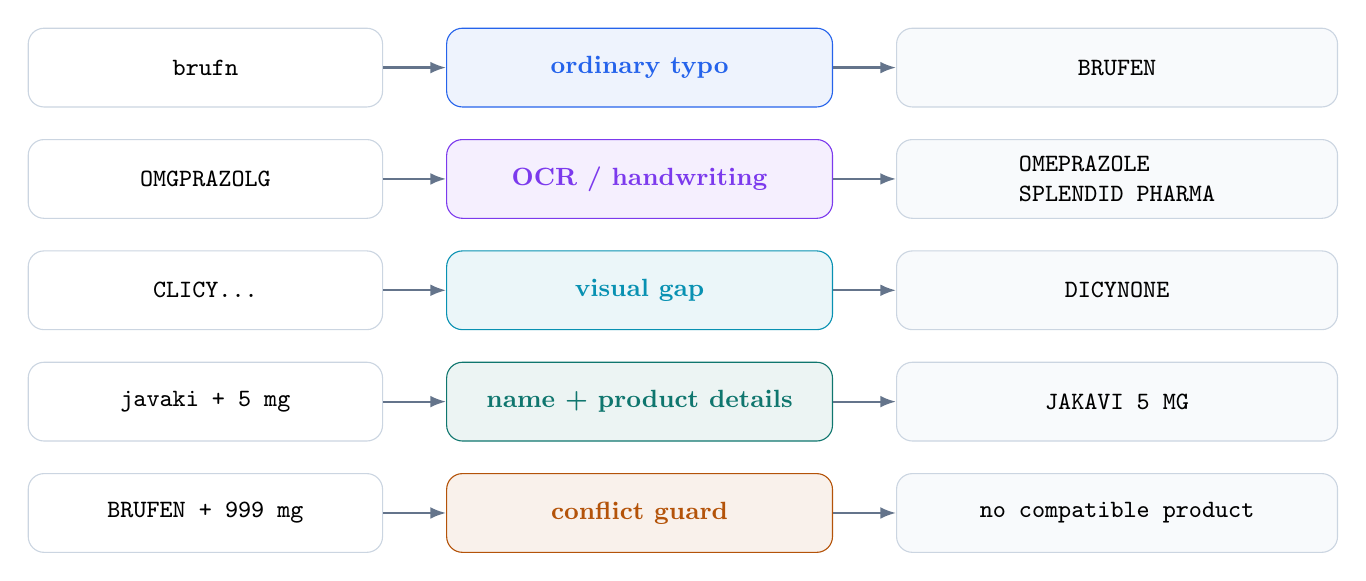
\begin{tikzpicture}[
  node distance=4mm and 8mm,
  source/.style={draw=Line,fill=white,rounded corners=2mm,minimum width=45mm,minimum height=10mm,align=left,font=\ttfamily\small},
  engine/.style={draw=#1,fill=#1!8,rounded corners=2mm,minimum width=49mm,minimum height=10mm,align=center,font=\headingfont\small\bfseries,text=#1},
  output/.style={draw=Line,fill=Pale,rounded corners=2mm,minimum width=56mm,minimum height=10mm,align=left,font=\ttfamily\small},
  arrow/.style={-{Latex[length=2mm]},thick,color=Muted}
]
\node[source] (i1) {brufn};
\node[engine=Blue,right=of i1] (e1) {ordinary typo};
\node[output,right=of e1] (o1) {BRUFEN};
\node[source,below=of i1] (i2) {OMGPRAZOLG};
\node[engine=Purple,right=of i2] (e2) {OCR / handwriting};
\node[output,right=of e2] (o2) {OMEPRAZOLE\\SPLENDID PHARMA};
\node[source,below=of i2] (i3) {CLICY...};
\node[engine=Cyan,right=of i3] (e3) {visual gap};
\node[output,right=of e3] (o3) {DICYNONE};
\node[source,below=of i3] (i4) {javaki + 5 mg};
\node[engine=Teal,right=of i4] (e4) {name + product details};
\node[output,right=of e4] (o4) {JAKAVI 5 MG};
\node[source,below=of i4] (i5) {BRUFEN + 999 mg};
\node[engine=Amber,right=of i5] (e5) {conflict guard};
\node[output,right=of e5] (o5) {no compatible product};
\foreach \n in {1,...,5}{\draw[arrow] (i\n) -- (e\n);\draw[arrow] (e\n) -- (o\n);}
\end{tikzpicture}
\end{center}

\begin{takeaway}[title=How to read the rest of this handbook]
Every rule is shown as \textbf{observed text} \mapstoex\
\textbf{allowed catalog interpretation}, followed by a positive example and
the safety condition that prevents it from becoming unrestricted fuzzy search.
\end{takeaway}

\section{How one query becomes a result}

\begin{center}
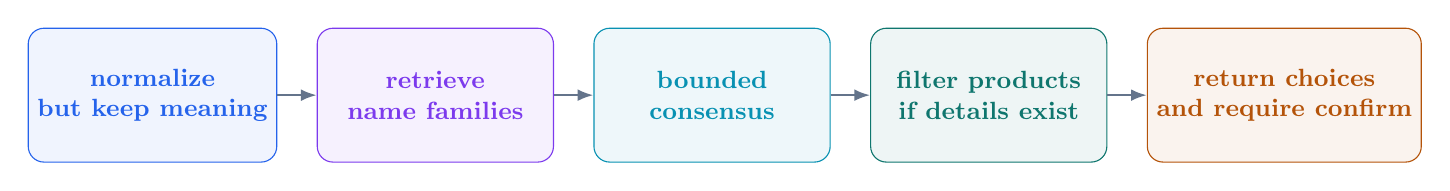
\begin{tikzpicture}[
  node distance=3mm and 5mm,
  step/.style={draw=#1,fill=#1!7,rounded corners=2mm,minimum width=30mm,
    minimum height=17mm,align=center,font=\headingfont\small\bfseries,text=#1},
  arrow/.style={-{Latex[length=2mm]},thick,color=Muted}
]
\node[step=Blue] (n) {normalize\\but keep meaning};
\node[step=Purple,right=of n] (r) {retrieve\\name families};
\node[step=Cyan,right=of r] (c) {bounded\\consensus};
\node[step=Teal,right=of c] (p) {filter products\\if details exist};
\node[step=Amber,right=of p] (s) {return choices\\and require confirm};
\draw[arrow] (n)--(r); \draw[arrow] (r)--(c); \draw[arrow] (c)--(p); \draw[arrow] (p)--(s);
\end{tikzpicture}
\end{center}

\subsection{Normalization keeps different evidence separate}

\begin{tabularx}{\textwidth}{@{}L{35mm}Y Y@{}}
\toprule
Input layer & Active normalization & Example and boundary \\
\midrule
Medicine name & Case, repeated spaces, punctuation, Arabic digits, common Arabic letter variants, elongation and diacritics are normalized; a compact key removes separators. & \observed{BRU-FEN} and \observed{brufen} share a lookup surface, but an explicit visual marker is detected before punctuation cleanup. \\
Product details & Arabic digits and decimal/thousands separators, micro symbols, dotted units, release abbreviations, multipacks and known aliases are normalized before parsing. & An Arabic-digit one-point-five MG dose normalizes to \observed{1.5 MG}; \observed{20 µg} $\mapsto$ \observed{20 UG}; malformed or zero doses fail closed. \\
Identity & Names use exact compact base-family keys; selected products use stable catalog IDs. Broad variant groups are display metadata only. & Two products with the same printed name remain separate if their catalog IDs, manufacturers, or prices differ. \\
\bottomrule
\end{tabularx}

\subsection{Retrieval and consensus rules}

Algorithm 5 builds the main candidate order from exact and alias evidence,
prefix/suffix and family-head indexes, tokens and character n-grams, bounded
deletes and edit distance, phonetic keys, skeleton keys, and the OCR/ligature
rules in the next section. Explicit visual-gap syntax takes its own branch.

{\RaggedRight Algorithm 6 then compares ten rankings: Algorithm 5 plus Jaro--Winkler,
Match Rating, WRatio, NYSIIS, BM25+character trigrams, SymSpell edit-distance
three, token-sort similarity, Soundex, and character-bigram Dice.
\par}

\begin{tabularx}{\textwidth}{@{}L{42mm}Y@{}}
\toprule
Consensus rule & Current behavior \\
\midrule
Base order & Algorithm 5 remains the base ranking. The Algorithm 6 rank-1 promotion gate is disabled. \\
External top-20 fill & If Algorithm 5 already supplies 20 rows, at most one absent family may replace the tail. If it supplies fewer rows, every vacant slot may be filled. Each external family still needs at least three retrievers, Levenshtein similarity $\geq .55$, and Jaro--Winkler $\geq .85$. \\
Learned OCR costs & Recorded as a diagnostic similarity only; they do not independently reorder results. \\
Decision state & Every row is low-confidence decision support with \texttt{confirmation\_required=true}. \\
\bottomrule
\end{tabularx}

\subsection{API and interface boundaries}

The API accepts 1--120 characters for the medicine query, up to 120 for
optional product details, and a result limit from 1 to 20. It hydrates display
fields by stable product ID first. The interface cache keeps raw visual-marker
semantics, so \observed{PANA DOL} and \observed{PANA...DOL} are different
requests. The static browser fallback is a separate search implementation and
is never reported as Python Algorithm 6 parity.

\section{Name reading rules}

\subsection{The direct OCR and handwriting registry}

These are the explicit observed-text-to-catalog mappings. Direction matters:
\observed{D} seen on paper is not always given the same cost as catalog
\observed{D} being read as two characters.

\rowcolors{2}{Pale}{white}
\begin{longtable}{@{}L{28mm}L{17mm}L{77mm}L{40mm}@{}}
\toprule
Observed $\mapsto$ catalog & Cost & Positive example & Main guard \\
\midrule
\endhead
I $\mapsto$ E & .45 & \caseflow{OMIPRAZOLI}{two I/E reads}{OMEPRAZOLE SPLENDID PHARMA} & Literal exact names stay protected \\
E $\mapsto$ I & .45 & \caseflow{PRESOLINEBLUE}{one E/I read}{PRISOLINE BLUE} & Original span consumed once \\
Y $\mapsto$ E & .45 & \caseflow{ROVADENY}{one Y/E read}{ROVADENE} & No transitive group merge \\
E $\mapsto$ Y & .45 & \caseflow{PERAZIDE}{one E/Y read}{PYRAZIDE} & Globally unique exact family \\
I $\mapsto$ Y & .45 & \caseflow{OXILOZIME}{one I/Y read}{OXILOZYME} & Bounded operation count \\
Y $\mapsto$ I & .45 & \caseflow{SALMOCALCYN}{one Y/I read}{SALMOCALCIN} & Bounded operation count \\
E $\mapsto$ G & .60 & \caseflow{INNOVAEAR}{one E/G read}{INNOVAGAR} & Direct retrieval only \\
G $\mapsto$ E & .60 & \caseflow{OMGPRAZOLG}{two G/E reads}{OMEPRAZOLE SPLENDID PHARMA} & Tail retrieval, not a global edit discount \\
CL $\mapsto$ D & .40 & \caseflow{CLICYNONE}{CL/D joined stroke}{DICYNONE} & Variable-length direct rewrite \\
D $\mapsto$ CL & .55 & \caseflow{BACTIDOR}{D/CL split stroke}{BACTICLOR} & Higher reverse cost \\
AL $\mapsto$ D & .45 & \caseflow{ALEPIDERM}{AL/D joined stroke}{DEPIDERM} & Global unique best family \\
D $\mapsto$ AL & .70 & \caseflow{DKDINE}{two D/AL reads}{ALKALINE} & Narrow depth-two exception \\
\bottomrule
\end{longtable}

\begin{proposedbox}[title=D / EL is not an implemented rule]
The team specifically raised \observed{D} versus \observed{EL}. The current
direct registry contains \observed{D/CL} and \observed{D/AL}, but not
\observed{D/EL}. It must remain labelled \textbf{proposed} until collision
analysis, positive cases, exact-name guards, and a downstream rerun justify it.
\end{proposedbox}

\subsection{All weighted spelling groups---not keyboard rules}

The general weighted edit score uses nine groups. Every different ordered
pair inside a group costs .45; the groups are similarity evidence, not one
canonical spelling.

\begin{tabularx}{\textwidth}{@{}L{27mm}L{28mm}rY@{}}
\toprule
Group & Members & Directions & Typical readings \\
\midrule
Consonant shape & C, K, Q & 6 & C$\mapsto$K, K$\mapsto$Q, Q$\mapsto$C \\
Hissing sound & S, Z & 2 & S$\leftrightarrow$Z \\
Lip sound & F, V & 2 & F$\leftrightarrow$V \\
Closed-lip shape & P, B & 2 & P$\leftrightarrow$B \\
Dental sound & D, T & 2 & D$\leftrightarrow$T \\
Soft/hard sound & G, J & 2 & G$\leftrightarrow$J \\
Joined hum shape & M, N & 2 & M$\leftrightarrow$N \\
Vowel handwriting & I, E, Y & 6 & I$\mapsto$E, E$\mapsto$Y, Y$\mapsto$I \\
Rounded vowel & O, U & 2 & O$\leftrightarrow$U \\
\bottomrule
\end{tabularx}

That is 26 weighted directions. Adding the two direct-only E/G directions
gives 28 observable one-character mappings, but E/G is deliberately excluded
from the global weighted metric so an incidental E/G alignment cannot disturb
an unrelated multi-error ranking.

Real QWERTY evidence is separate: horizontal and vertical neighboring keys
may reverse exactly one keyboard substitution. The normal keyboard generator
is limited to names of length 4--16; a separate exact short path handles
length 3. The older 800-case ordinary benchmark covers horizontal neighbors;
the new hard suite also separates arbitrary substitution from keyboard evidence.

\begin{safetybox}[title=Why E/G is kept separate]
E belongs to the I/E/Y handwriting group and G belongs to G/J. Joining the
groups would incorrectly imply I, Y, E, G, and J are all interchangeable.
The implementation therefore applies E/G only through bounded directional
evidence and never through transitive canonicalization.
\end{safetybox}

\subsection{All OCR digits, ligatures, and phonetic rewrites}

\begin{tabularx}{\textwidth}{@{}L{30mm}Y@{}}
\toprule
Registry & Every active observed $\mapsto$ catalog direction \\
\midrule
OCR digits (9) & 0$\mapsto$O; 1$\mapsto$I; 1$\mapsto$L;
2$\mapsto$Z; 3$\mapsto$E; 4$\mapsto$A; 5$\mapsto$S;
6$\mapsto$G; 8$\mapsto$B. Digits 7 and 9 have no expansion. \\
Ligatures (14) & RN$\mapsto$M; M$\mapsto$RN; CL$\mapsto$D;
D$\mapsto$CL; LI$\mapsto$H; H$\mapsto$LI; RI$\mapsto$N;
AL$\mapsto$D; NN$\mapsto$M; VV$\mapsto$W; W$\mapsto$UU;
IV$\mapsto$N; IA$\mapsto$A; II$\mapsto$U. \\
Phonetic (21) & PH$\mapsto$F; F$\mapsto$PH; CK$\mapsto$K;
K$\mapsto$CK; X$\mapsto$KS; KS$\mapsto$X; CKS$\mapsto$X;
QU$\mapsto$KW; KW$\mapsto$QU; QU$\mapsto$CW; GH$\mapsto$G;
TH$\mapsto$T; TH$\mapsto$S; GHT$\mapsto$T; WH$\mapsto$W;
SH$\mapsto$CH; CH$\mapsto$SH; TION$\mapsto$SHUN;
Y$\mapsto$I; I$\mapsto$Y; Y$\mapsto$EE. \\
\bottomrule
\end{tabularx}

All 14 ligature directions participate in bounded one-step exact retrieval.
The mixed ligature-plus-vowel generators intentionally use only the first six
directions: RN$\leftrightarrow$M, CL$\leftrightarrow$D, and
LI$\leftrightarrow$H. A special N$\mapsto$RI expansion exists only for exact
three- and four-character family retrieval. None of these one-step outputs is
recursively fed back through the same registry.

\subsection{Bounded long phonetic collapse plus one ordinary error}

Two long collapses need one extra, tightly bounded path because an OCR word may
contain both the collapse and one ordinary typo:

\begin{tabularx}{\textwidth}{@{}L{28mm}L{39mm}Y@{}}
\toprule
Rule & Concrete cases & Boundary that keeps it safe \\
\midrule
CKS$\mapsto$X plus one edit & \observed{CKSEFO}$\mapsto$XEFO;
\observed{XSSACKS}$\mapsto$ASSAX & Exact catalog lookup only; the complete
family set must have at most four members. \\
GHT$\mapsto$T plus one edit & \observed{GHTAXA}$\mapsto$TADA, TALA;
\newline\observed{OGHTA}$\mapsto$OTAL, VOTA, YOTA & Query length 5--20; the character
created by GHT$\mapsto$T cannot be edited again. \\
Rank preservation & \observed{OGHTAL}$\mapsto$OTAL remains rank 1 & The rule
adds evidence and reserves hidden tail slots; it never promotes itself to rank
1 or moves an already-visible family to the tail. \\
\bottomrule
\end{tabularx}

This path is intentionally not generalized to every phonetic rewrite. It was
added only after the hard ambiguity suite found equal protected-span evidence
that the exact-only phonetic lookup could not retrieve. Algorithm 6 also
protects these bounded tail rows from consensus eviction.

\subsection{Skeleton, phonetic, and chain keys}

\begin{tabularx}{\textwidth}{@{}L{31mm}Y L{49mm}@{}}
\toprule
Mechanism & Exact transformation & Concrete boundary \\
\midrule
Skeleton key & PH$\mapsto$F; [CQK]$\mapsto$K;
[PV]$\mapsto$B; [SZ]$\mapsto$S; remove A/E/I/O/U/Y;
collapse repeats. & \observed{PAVA} becomes skeleton \observed{B}, while
\observed{FAVA} becomes \observed{FB}. F is not merged with B/P/V. \\
Phonetic key & PH$\mapsto$F, CK$\mapsto$K, GH$\mapsto$G;
[BPFV]$\mapsto$P; [DT]$\mapsto$T; [CGKQ]$\mapsto$K;
[SZ]$\mapsto$S; J$\mapsto$G; remove vowels; collapse repeats. & The ordered
pipeline is a coarse retrieval key; full-name edits still decide ranking. \\
Visual chain groups & AOUE; ILT; HNBR; MN; GQY; UVW; FTL; ECO. & Used only
inside named bounded multi-operation chains, not as a global substitution cost. \\
Sound chain groups & BP; DT; GK; SZ; FV; CKQ. & At most the operation count
allowed by the named chain generator; not an unrestricted phonetic search. \\
Visual-gap key & PH$\mapsto$F, CK$\mapsto$K, QU$\mapsto$K,
GH$\mapsto$G, C/Q$\mapsto$K, repeats collapsed. & This is the separate
fragment projection used by the next section; target widths stay measurable. \\
\bottomrule
\end{tabularx}

\subsection{The 27 explicit source aliases}

These are literal compact-query entries in the inherited base retriever. Each
points to a source retriever target, which may be an exact base family or a
broader prefix/display head. In particular, PANADOL is a source target rather
than a standalone exact base family. The entries are not learned from search
results and do not create a general sound-alike rule.

{\small
\begin{tabularx}{\textwidth}{@{}Y Y Y@{}}
\toprule
Alias $\mapsto$ source target & Alias $\mapsto$ source target & Alias $\mapsto$ source target \\
\midrule
BANADOL$\mapsto$PANADOL & BANDOL$\mapsto$PANADOL & PANDOL$\mapsto$PANADOL \\
PNDL$\mapsto$PANADOL & PANDL$\mapsto$PANADOL & PANADL$\mapsto$PANADOL \\
PANADOLE$\mapsto$PANADOL & BANADOLE$\mapsto$PANADOL & BANADOLCOLD$\mapsto$PANADOL \\
PANDOLCOLD$\mapsto$PANADOL & BANDOLCOLD$\mapsto$PANADOL & OGMENTIN$\mapsto$AUGMENTIN \\
OGMNTIN$\mapsto$AUGMENTIN & AUGMNTIN$\mapsto$AUGMENTIN & AUGMANTIN$\mapsto$AUGMENTIN \\
FOLTARIN$\mapsto$VOLTAREN & VOLTARIN$\mapsto$VOLTAREN & FOLTAREN$\mapsto$VOLTAREN \\
BRUFN$\mapsto$BRUFEN & BRFN$\mapsto$BRUFEN & BRUFIN$\mapsto$BRUFEN \\
BROFEN$\mapsto$BRUFEN & KETOFN$\mapsto$KETOFAN & KETOFEN$\mapsto$KETOFAN \\
NEKSIUM$\mapsto$NEXIUM & NEKSUM$\mapsto$NEXIUM & NEXUM$\mapsto$NEXIUM \\
\bottomrule
\end{tabularx}
}

\subsection{Budgets that keep the OCR rules bounded}

\begin{itemize}
\item Fewer than 4 visible name characters: no direct OCR rewrite.
\item 4--5 characters: at most one registered direct confusion.
\item 6--24 characters: at most two registered direct confusions.
\item More than 24 characters: the direct rewrite recursion is disabled.
\item The ordinary public variant-list call retains at most 512 deterministic
variants. Exact-family retrieval, corrected-prefix retrieval, and the global
promotion audit deliberately enumerate the full reachable set without that cap.
\item Rewrites consume the original span. One letter cannot become E, then G,
then another group in the same path.
\item Ambiguous exact families may be retrieved and shown. Global minimum-cost
uniqueness is required only when the direct-grapheme layer tries to promote one
family to rank 1; that candidate must be in the first 12 and within the live
.65 score gap. A literal exact catalog name is restored above confusion-only
alternatives.
\end{itemize}

\subsection{How a family enters the candidate pool}

\begin{longtable}{@{}L{34mm}L{68mm}L{64mm}@{}}
\toprule
Channel & What the engine opens & Bound that prevents flooding \\
\midrule
\endhead
Exact family & Exact compact catalog-family key. & Literal equality is
protected again after ordinary promotions. \\
Prefix and suffix & Prefix and reverse-suffix indexes of length 2--12. &
Normal query prefix retrieval starts at 3 characters; suffix at 4. \\
Rare character grams & Up to four rare 4-grams; if the pool is below 160,
up to five rare 3-grams. & Common buckets do not receive the same expansion. \\
Skeleton and phonetic & Exact keys and key prefixes of length 3--10. & A key
match is retrieval evidence; the full name still supplies edit and position scores. \\
Delete index & No deletes below length 4; one delete at 4--7; two at 8 and
above. & Retained delete key length at least 3; a query delete bucket over 650
families is not opened. \\
First-character expansion & E$\mapsto$G and G$\mapsto$E only, before prefix
and length-index lookup. & The nine broader confusion groups stay scoring
evidence; they do not expand the first-character pool. \\
Compatible-length scan & Query length 4--12, only when the base search is weak
or uncertain. Radius 3, or 0 when the core pool already has at least 220 rows. &
Plausible first character required; at most 2,200 family IDs. \\
Bounded nearest & Query length 3--16; radii 1, 2, 3, 4 for lengths 3, 4--6,
7--9, 10--16. & Only minimum-distance ties; at most 12 families; plausible
first-character evidence required. \\
Short rescue & Exact length-3 keyboard neighbor; two-deletion frame for length
3--4; consonant/phonetic frame for length 3--7; equal 2-character edge; short
visible head. & Short frame keeps 8, raw distance $\leq3$, weighted distance
$\leq2.25$; visible-head surfacing keeps 4 and is not automatic rank 1. \\
Family head & Shared first token of length at least 4, supported by at least
two catalog families and common manufacturer evidence. & Normal head rescue
uses query length 5--18 and validated head distance at most 2. \\
One-step evidence variants & Exactly one OCR digit, leading swap, ligature,
phonetic rewrite, stuttered prefix, transposition, or keyboard neighbor. &
Evidence variant limit 12; mixed ligature/transposition limit 48; normal
keyboard names length 4--16. \\
Exact multi-operation chains & Visual+sound, two visual+delete,
transpose+delete, ligature+vowel, ligature+vowel+transpose,
transpose+vowel+delete, vowel+sound+delete, keyboard+vowel+delete, and short
digit+vowel/sound. & Each chain has its own length, depth, transformed-distance,
rank, score-gap, and uniqueness gate; the 17 promotion policies are below. \\
Corrected prefix & A direct rewrite becomes an exact prefix of a longer
catalog family. & Query length 6--24, total cost $\leq1.40$, prefix bucket
$\leq4$, result limit at least 2; tail visibility only, never rank 1. \\
Context-clean second pass & Remove recognized strength/unit/form noise and run
the base name search again. & Cleaned name must differ and retain at least 3
characters; short weak prefixes are blocked and leading numeric brands remain. \\
Legacy unreadable modes & Structured \texttt{before}, \texttt{middle}, and
\texttt{after} modes filter merged A5 candidates by visible anchors. & Target
must be longer than visible text; this older dict mode is separate from the
explicit Algorithm 6 gap grammar in the next section. \\
\bottomrule
\end{longtable}

\subsection{Edit costs, prefilter, and full family score}

\begin{tabularx}{\textwidth}{@{}L{43mm}L{21mm}Y@{}}
\toprule
Observed operation & Cost & Important scope \\
\midrule
Insertion; deletion; ordinary substitution & 1.00 & Default raw spelling error. \\
One of the 26 weighted-group directions & .45 & Global weighted comparison. \\
Other vowel-to-vowel substitution & .70 & Used only when the pair did not already receive .45. \\
Adjacent transposition & .55 & Raw Damerau still counts one edit. \\
Listed OCR digit$\mapsto$letter & .45 & OCR-visual comparison only. \\
Direct CL/D, AL/D, I/E/Y, or E/G operation & Registry cost & Bounded direct evidence; E/G is not a global discount. \\
Repeated arbitrary character & deletion cost & Only a duplicated 2- or 3-letter prefix has a special exact stutter rule. \\
\bottomrule
\end{tabularx}

The broad prefilter is deterministic and bounded. With prefix \(P\), suffix
\(S\), character-gram Jaccards \(G_2,G_3,G_4\), skeleton/phonetic
similarities \(K_s,K_p\), subsequence \(Q\), weighted edit \(E_w\), position
\(X\), and length coverage \(C\):

\[
S_{\mathrm{pre}}=1.35P+.65S+.55G_2+1.20G_3+1.00G_4
 +.70K_s+.65K_p+.35Q+.90E_w+.45X+.25C.
\]

The main shortlist keeps 45 family rows; the edge path reserves 15. A full
candidate is then scored as

\[
S_{\mathrm{family}}=1.25I+.58E+.52E_w+.16P+.10S+.10G_2+.18G_3
 +.16K_s+.14K_p+.10Q+.24X+.16C,
\]

plus bounded first-character, close-length, prefix, and weighted-position
bonuses and weak-short penalties. Normal admission is at .62. The narrow
positional rescue may enter from .58 only with the same first character,
position agreement at least .40, and length coverage at least .70.

The original base search, cleaned-context pass, and rescue search are merged
with different rank-aware contributions:
\[
S_{\mathrm{base}}=.72\min(s,1)+\frac{.32}{r+2},\quad
S_{\mathrm{context}}=.84\min(s,1)+\frac{.40}{r+2}+.05,\quad
S_{\mathrm{rescue}}=s+\frac{.18}{r+1}.
\]
Non-confident base evidence is multiplied by .90; base/context agreement adds
.06 and base/rescue agreement adds .08. Those scores form a candidate order,
then only the named gates below may change it.

\subsection{When a candidate may move up: every promotion family}

\begin{takeaway}[title=What ``promotion'' means]
A promotion is a \textbf{bounded reorder}, not a confident medicine selection.
The family must already have been retrieved, and every condition of one named
gate must pass; otherwise the order stays unchanged. Here, ``rank'' means the
family's position immediately before that gate runs---not its Algorithm 2
external rank or rescue rank. Literal exact-name restoration runs after the
ordinary promotion chain, and every final result still requires confirmation.
\end{takeaway}

\begin{longtable}{@{}L{38mm}L{74mm}L{54mm}@{}}
\toprule
Promotion family & What may move & Main blocker \\
\midrule
\endhead
Four core corrections & Dual closer; pure deletion; closer single-token over
multi-token; validated variant head. & Exact top or any failed raw, score,
token, group, or head-distance conjunct. \\
Unique and contained nearest & Unique first-three candidate with raw
$\leq4$, gain $\geq2$, gap $\leq.75$; or rank-2 contained candidate raw
$\leq1$, gain 1, gap .25. & Equal nearest families remain ambiguous. \\
Preserved-top nearest release & Rank 2 passes a preserved top only with the
required raw, weighted, edge, and score dominance. & A tie or missing strict
improvement keeps the incumbent. \\
Exact ligature & Unique exact ligature evidence among the first five. & New
variable-length direct candidates are limited to original ranks 2--3;
raw-worse AL$\mapsto$D is blocked. \\
Weighted edge & Unique tied/near rank-2 or rank-3 family with weighted gain
(.50 or .70), edge gain, and bounded gap (.25 or .40). & Full-name and
historical regression guards block broad visual overpromotion. \\
Exact-key Pareto & Exact skeleton/phonetic candidate no worse on weighted,
position, edge, and dual evidence; rank at most 3, gap at most .15. & Nonunique
key or any worse signal. \\
Transposition & Unique exact one-swap candidate at rank 2--3, or a dual rank-2
extension, with raw distance at most 1 and bounded gap. & Short/nonunique swap
or worse weighted evidence. \\
Keyboard & Exact one-key neighbor at rank 2; weighted extension requires gain
at least .25 and gap at most .15. & Cannot erase an equally supported collision. \\
Narrow tie breakers & Exact visual edge, phonetic-position, shifted-edge,
visual-distance, and skeleton-position evidence. & Each requires its own
unique edge/position/key gain and a score gap between .05 and .40. \\
Score-chain release & A chain candidate already stronger on bounded
score/raw/weighted evidence may be released from a preserved top. & Retrieval
reason alone is never enough. \\
Stutter prefix & Removing one duplicated initial 2- or 3-character block
produces exactly one catalog family. & Multiple targets or arbitrary internal
repeats do not receive this rule. \\
Exact phonetic rewrite & One exact one-step phonetic family inside the first 5. &
Competing sound-alikes remain visible rather than becoming false uniqueness. \\
Strict full name & Rescue-only family, query length at least 5, raw at most 3,
weighted gain at least .35, edge gain .05, rescue rank at most 5, gap .35. &
Exact/prefix/contained incumbents and failed edge evidence. \\
Family-head and character Pareto & Validated family head, short visible head,
ordered-character head, bounded head, or Pareto-character evidence. & Shared
manufacturer, LCS, edit, edge, score, uniqueness, and full-name guards. \\
Two-sided anchor & Unique family supported at both name edges, gap at most .40,
with weighted/LCS/edge checks. & Equal support does not reorder. \\
Direct grapheme & Globally unique minimum-cost exact target within rank 12,
live gap at most .65, weighted no worse, normally raw disadvantage at most 1. &
Literal exact query, ambiguity, transitive path, raw-worse AL$\mapsto$D, or any
failed conjunct. \\
Exact-name restoration & Literal exact compact catalog family returns above
confusion-only alternatives. & Legacy unreadable mode is a separate branch. \\
Corrected-prefix/post-repair & Longer corrected-prefix families are tail
surfaced; three narrow repairs protect a strict Pareto chain, an external-rank
tie, or one constrained top-5 chain family. & No general rank-1 jump. \\
Algorithm 6 consensus & Algorithm 5 stays the base order; the learned rank-1
gate is disabled. External families need 3 sources, Levenshtein .55, and
Jaro--Winkler .85. & One replacement if A5 is full; only vacant slots are
filled if it is underfull. \\
Final decision & Every returned family remains low-confidence decision support. &
\texttt{needs\_clarification=true} and \texttt{confirmation\_required=true}. \\
\bottomrule
\end{longtable}

\Needspace{.38\textheight}
\textbf{Worked examples from frozen tests.} These rows show gates that actually
fired in the preserved final run; they illustrate the rules above rather than
adding new rules.

\begin{tabularx}{\textwidth}{@{}L{34mm}L{45mm}L{29mm}Y@{}}
\toprule
Promotion family & Observed input $\mapsto$ expected family & Frozen result & Why the move was allowed \\
\midrule
Unique nearest & \observed{VVEIORN} $\mapsto$ WE IORN & Expected family finished rank 1 & One unique near family; raw distance at most 4, gain at least 2, and gap at most .75. \\
Exact ligature & \observed{RIEOMUNE} $\mapsto$ NEO MUNE & Expected family finished rank 1 & One exact ligature target, also the unique nearest family, with dual retrieval and no worse weighted distance. \\
Weighted edge & \observed{CLMAE} $\mapsto$ DMAE & Expected family finished rank 1 & Raw-distance tie, but DMAE was the unique weighted winner and had sufficient edge evidence. \\
Strict full name & \observed{MELTAOIVIN} $\mapsto$ MELATONIN & Expected family finished rank 1 & Rescue-only target with raw distance 3 or less plus weighted and edge gains; no exact/prefix incumbent blocked it. \\
Validated family head & \observed{UROSOLVINYN} $\mapsto$ UROSOLVINE N & Expected family finished rank 1 & One validated family head was within two edits, closer than the incumbent, and began with the same character. \\
Direct grapheme & \observed{CACLEX} $\mapsto$ CADEX & Expected family finished rank 1 & Globally unique minimum-cost exact target, already within rank 12, with gap at most .65 and no worse weighted distance. \\
\bottomrule
\end{tabularx}

\begin{safetybox}[title=The blocker is part of the rule]
\observed{MYLANO} can reach both MELANO and MILANO at equal minimum cost, so
both must remain visible and neither receives a deterministic grapheme
promotion. Conversely, literal \observed{CEFIX} must remain rank 1 even when a
confusion-only alternative exists. A positive example without its ambiguity
and exact-name guards would be an incomplete description of the rule.
\end{safetybox}

\subsection{The 17 exact-chain promotion policies}

Each row starts only after its operation chain reaches an exact catalog key.
Let \(r\) be current rank, \(g=S_{\mathrm{top}}-S_{\mathrm{candidate}}\), and
\(d\) be the candidate raw-distance disadvantage. ``Exact key'' means a skeleton/phonetic
advantage; ``dual'' means base and rescue support.

{\scriptsize
\begin{longtable}{@{}rL{49mm}L{34mm}L{65mm}@{}}
\toprule
ID & Chain & Rank/gap/raw bound & Additional evidence \\
\midrule
\endhead
1 & Ligature+vowel+transpose, core & \(r\leq5,g\leq.40,d\leq1\) & Unique; normal head protection. \\
2 & Ligature+vowel+transpose, extension & \(r\leq5,g\leq.75,d\leq1\) & Preserve correction; relaxed head protection. \\
3 & Ligature+vowel, core & \(r\leq5,g\leq.40,d\leq0\) & Unique; candidate cannot be raw worse. \\
4 & Ligature+vowel, distance extension & \(r=2,g\leq.05,d\leq1\) & Preserve an existing correction. \\
5 & Ligature+vowel, edge extension & \(r=2,g\leq.15,d\leq1\) & Edge no worse; preserve correction. \\
6 & Ligature+vowel, multi-chain extension & \(r\leq5,g\leq.40,d\leq1\) & At least two exact-chain reasons. \\
7 & Two visual steps + one sound step & \(r\leq5,g\leq.10,d\leq1\) & Unique and dual support. \\
8 & Visual+sound exact-key extension & \(r=2,g\leq.40,d\leq0\) & Exact key and weighted no worse. \\
9 & Visual+sound dual extension & \(r\leq4,g\leq.15,d\leq0\) & Dual, weighted no worse, relaxed head protection. \\
10 & Keyboard+vowel+delete, core & \(r\leq5,g\leq0,d\leq1\) & Exact-key advantage. \\
11 & Keyboard+vowel+delete, extension & \(r\leq3,g\leq.25,d\leq1\) & Exact key and weighted no worse. \\
12 & Two visual steps + target delete & \(r\leq3,g\leq.02,d\leq1\) & Position no worse. \\
13 & Visual+delete multi-chain & \(r\leq3,g\leq.15,d\leq0\) & Weighted no worse; at least three chain reasons. \\
14 & Transposition+target delete & \(r\leq3,g\leq.25,d\leq0\) & Exact key and weighted no worse. \\
15 & Transposition+vowel+delete & \(r\leq5,g\leq0,d\leq0\) & Preserve correction; relaxed head protection. \\
16 & Vowel+sound+delete, short & \(r=2,g\leq.25,d\leq2\) & Query length 3--4; weighted no worse; two reasons. \\
17 & Vowel+sound+delete, multi-extension & \(r=2,g\leq.10,d\leq2\) & Query length 3--4; exact key; two reasons. \\
\bottomrule
\end{longtable}
}

The list describes promotion policies, not every retrieval route. Short
OCR+vowel/sound and the short two-deletion frame also retrieve exact families,
but they flow through the short/evidence and baseline-preservation gates.

\section{Visual-gap rules}

The visual-gap mode is for a user who can read fragments but not the text
between them. It is a distinct query grammar, not a general typo symbol.

\begin{tabularx}{\textwidth}{@{}L{32mm}L{43mm}Y@{}}
\toprule
Mode & Example & Meaning \\
\midrule
Leading gap & \observed{...DOL} & At least one hidden target character before DOL. \\
Trailing gap & \observed{PANA...} & At least one hidden target character after PANA. \\
Internal gap & \observed{PANA...DOL} & PANA and DOL occur in order with at least one real hidden target character between them. \\
Both edges & \observed{...INADC...} & Hidden text exists at both edges; the exact family CLINDACIN ADCO is recoverable. \\
Multiple gaps & \observed{DI...CY...ONE} & Up to four retained fragments, in order. \\
Whitespace shorthand & \observed{PANA DOL} & Two to four alphabetic fragments; joining may be zero-width. \\
\bottomrule
\end{tabularx}

\begin{takeaway}[title=Accepted explicit markers]
Two or more dots, the ellipsis character, one or more asterisks, one or more
question marks, or two or more underscores. Punctuation-separated words that
do not match this grammar stay ordinary spelling queries. A \textbf{single}
\observed{*} or \observed{?} is therefore an active gap marker; this exact
boundary is covered by the generated marker-glyph tests.
\end{takeaway}

\subsection{Four matching stages}

\begin{enumerate}
\item \textbf{Literal ordered fragments}: exact visible text in the required order.
\item \textbf{Fixed grapheme projection}: PH/F, CK/K, QU/K, GH/G, C/Q/K, repeats.
\item \textbf{Bounded OCR confusion}: the direct registry above, active only
for 5--24 visible characters; one confusion below 8 visible characters and at
most two from 8 upward, with cost budgets 1.00 and 1.40.
\item \textbf{One ordinary visible edit}: insertion, deletion, or substitution
only when total visible text is at least five characters and every fragment
has at least two characters.
\end{enumerate}

Every explicit marker must correspond to at least one target character. The
matcher backtracks across repeated fragment occurrences, preserves the exact
matched base family, and reports hidden characters and coverage on the target
side. All returned rows require confirmation.

\begin{tabularx}{\textwidth}{@{}L{42mm}L{50mm}Y@{}}
\toprule
Test & Expected behavior & Rule being protected \\
\midrule
\observed{AT...OL} & ATENOLOL is recoverable using the final OL, not the first one & repeated-occurrence backtracking \\
\observed{PANA...DOL} vs PANADOL & exact PANADOL is rejected & internal marker must hide a character \\
\observed{...PANADOL} vs PANADOL & exact PANADOL is rejected & leading marker must hide a character \\
\observed{BRU...} + 600 mg & exact BRUFEN base is selected, not a broad sibling group & visual exact-family identity \\
\observed{VIT\_\_3} & visual mode stays visual; bare 3 is not silently parsed as product context & cross-mode isolation \\
\end{tabularx}

\subsection{What the new visual benchmark actually tests}\label{sec:visual-benchmark}

\begin{tabularx}{\textwidth}{@{}L{39mm}r Y L{42mm}@{}}
\toprule
Cohort & Rows & What is varied & Example \\
\midrule
Structural positives & 240 & Leading, trailing, internal, both-edge, multi-fragment, and whitespace shorthand; 40 each & \observed{...AGLOBE} $\mapsto$ DEXAGLOBE; \observed{LUM OIL} $\mapsto$ LUMIERE HAIR OIL \\
OCR/glyph composition & 54 & One OCR confusion plus a gap; every accepted marker glyph & \observed{WOMYGR...} $\mapsto$ WOMEGRANTY \\
Numeric visual names & 20 & Digits belong to the medicine name and must not become product strength & \observed{VITA...D3K2} $\mapsto$ VITAMIN D3 K2 \\
Exact ambiguity & 30 & Every exact base family satisfying the same mask is labelled relevant & \observed{PRE...RAX} keeps PREGORAX and PRETERAX \\
Safety boundaries & 80 & Zero-width explicit gaps, short-confusion floor, punctuation collisions, and numeric shorthand isolation & \observed{CEVI...ANO} must not match exact CEVIANO \\
\bottomrule
\end{tabularx}

The 424 rows were generated before execution from exact catalog base-family
surfaces and split by family-stable hashes (338 development, 86 holdout).
The oracle stores both the selected exact source family and the complete set
of exact families satisfying the mask. Evaluation reads
\texttt{matched\_family\_key}; the broad display group never earns credit.

\section{Product-detail rules}

Optional product details never replace the medicine-name evidence. They filter
or reorder products only inside a bounded set of plausible exact families.

\subsection{Numeric evidence}

\begin{tabularx}{\textwidth}{@{}L{39mm}Y L{48mm}@{}}
\toprule
Rule & What is recognized & Safety behavior \\
\midrule
Qualified strength & mg, mcg/ug, g, kg, IU/U, MIU, percent, and safe unit conversions & Explicit zero or malformed magnitude fails closed. \\
Concentration & numerator/denominator including mL, L, g, microlitre, and time denominators & Exact printed tuple wins; a scaled-equivalent ratio is compatible but not an equal exact tie. \\
Combination strength & repeated components, shared denominators, mixture ratios, colon ratios & All supplied components must agree. \\
Presentation quantity & container weight/volume such as 50 g cream & Quantity alone is weak; quantity plus matching structural form may select. \\
Bare number & \observed{600} with a plausible family; or number plus form & May express strength or pack count, but only through bounded hypotheses. \\
Package count & tablets, capsules, doses, actuations, patches, suppositories, pens, syringes, cartridges, multipacks & Every supplied count must be satisfied; one matching count cannot hide an extra conflicting count. \\
\bottomrule
\end{tabularx}

\Needspace{52mm}
\subsection{Form, route, release, and container}

\begin{itemize}
\item Form aliases distinguish tablet, capsule, liquid, cream, gel, ointment,
drops, spray, suppository, solution, vial, ampoule, syringe, pen, cartridge,
and other catalog forms.
\item Route keeps oral/topical/ophthalmic/etc. evidence and preserves injection
subtypes such as IV, IM, and SC when explicitly supplied.
\item Release terms distinguish immediate products from SR, XR, ER, CR, MR,
retard, extended-release, and dotted abbreviations.
\item If the query supplies a category and the product lacks or contradicts
that metadata, the product is not labelled compatible.
\end{itemize}

\subsection{Family admission and selection}

\begin{tabularx}{\textwidth}{@{}L{43mm}Y@{}}
\toprule
Situation & Active rule \\
\midrule
Exact medicine name & Hard boundary: product context cannot jump to another base family or a sibling folded into a broad display group. \\
Ordinary nonexact name & Rank 1 is admitted; ranks 2--3 require every available diagnostic to pass raw distance $\leq2$ and similarity $\geq.60$; rank 4+ is excluded. \\
Visual-gap name & First three structurally matched exact base families are eligible; broad variant siblings are not opened automatically. \\
Strong exact numeric evidence & Compatible products can reorder admitted families; incompatible name-only rows do not leak into a successful product selection. \\
Weak form/presentation evidence & May filter, but cannot freely pull a distant medicine above a stronger name match. \\
No compatible product & Return the admitted medicine name(s) with an explicit no-compatible decision; never invent a product. \\
Product tie & Keep every genuinely tied stable product ID, subject to the public result limit. \\
\bottomrule
\end{tabularx}

\begin{resultbox}[title=Three examples that define the intended behavior]
\caseflow{javaki + 5 mg}{rank-2 name plus exact strength}{JAKAVI 5 MG}\\
\caseflow{brufen + 600}{exact family lock plus strength}{three legitimate BRUFEN 600 MG ties}\\
\caseflow{brufen + 600 tab}{strength plus form/package evidence}{one compatible BRUFEN tablet product}
\end{resultbox}

\subsection{Numeric aliases and very short prefixes}

Exact commercial aliases beginning with numbers are indexed by exact base
family. The longest exact alias wins, an unknown suffix blocks the rescue, and
visual-gap mode disables numeric-alias and short-prefix shortcuts. The special
numeric-only alias \observed{1 2 3} intentionally returns both exact families
and requires confirmation. A one- or two-letter prefix such as
\observed{x + 500 tab} may use context only when the family set is small and
the numeric/form evidence is compatible; a broad or conflicting set abstains.

\section{Safety rules around every result}

\begin{tabularx}{\textwidth}{@{}L{43mm}Y@{}}
\toprule
Guard & What it prevents \\
\midrule
Literal exact-name protection & A confused spelling cannot outrank the exact catalog spelling entered by the user. \\
Global uniqueness before promotion & An OCR rewrite shared by multiple families cannot become a confident single correction. \\
Original-span non-transitivity & Overlapping visual groups cannot chain one character through several identities. \\
Exact base-family identity & Product details and visual matches cannot open unrelated siblings from a broad display group. \\
All supplied details must match & One correct strength or count cannot hide a conflicting route, release, container, or second count. \\
Stable product IDs & Duplicate commercial-name strings remain distinct products with their own price/company/record. \\
Visual-mode isolation & Gap punctuation cannot be cached or normalized into an ordinary/numeric-alias query. \\
Always confirm & Every result is decision support, never autonomous clinical selection. \\
\bottomrule
\end{tabularx}

\section{The new test sets}

The selected name-rule cases below are organized as five separate claims. The
complete 336-row registry remains the source-to-test crosswalk for rules that
could not enter these catalog-derived files. Accuracy misses, hard safety
failures, broad collision diagnostics, and source-boundary failures are never
pooled into one reassuring percentage.

\begin{center}
\metric{3,284}{hard name-accuracy rows}{Blue}\hfill
\metric{272}{hard ambiguity/exact guards}{Amber}\hfill
\metric{100+11}{diagnostic + source rows}{Purple}
\end{center}

\subsection{Hard name-reading standard: five frozen files}

\begin{tabularx}{\textwidth}{@{}L{47mm}rL{35mm}Y@{}}
\toprule
File & Rows & Verdict type & What it isolates \\
\midrule
\path{name_reading_atomic_accuracy.csv} & 1,724 & Accuracy & One controlled
mapping, one missing ordinary-error channel, or one declared alias. \\
\path{name_reading_composed_accuracy.csv} & 1,560 & Accuracy & Exactly two
non-overlapping operations across 13 composition signatures. \\
\path{name_reading_collision_safety.csv} & 272 & Hard gate & 100 atomic
query collisions, 100 same-fingerprint composed collisions, and 72 literal
exact-name guards. \\
\path{name_reading_cross_channel_diagnostics.csv} & 100 & Diagnostic & A
broader query collision reached through unlike two-operation paths; relevant
breadth is measured but not mislabelled equal evidence. \\
\path{name_reading_source_boundaries.csv} & 11 & Hard gate & Length/depth,
non-transitivity, E/G-only first-character scope, deterministic order, and the
default 512-variant cap. \\
\bottomrule
\end{tabularx}

\begin{takeaway}[title={Four difficulty levels, four different claims}]
\textbf{L1 atomic} and \textbf{L2 composed} report Hit@1, Hit@5, Hit@20, and
MRR; every miss stays in the denominator. \textbf{L3 strict ambiguity} must
show every family generated by the same declared evidence fingerprint, while a
literal exact query must remain rank 1. Cross-rule L3 collisions are breadth
diagnostics because their paths and costs differ. \textbf{L4 source boundaries}
are direct pass/fail contracts. Wrong runtime identity or missing confirmation
invalidates any row regardless of rank.
\end{takeaway}

\subsection{What ``hard'' means in this suite}

\begin{tabularx}{\textwidth}{@{}L{43mm}Y@{}}
\toprule
Coverage layer & Exact construction \\
\midrule
Source inventory & 71 deduplicated observed$\mapsto$catalog mappings from the
weighted groups, direct graphemes, OCR digits, ligatures, and phonetic
registry; 27 declared source aliases; and four previously underrepresented
ordinary channels: arbitrary insertion, general substitution, whitespace, and
punctuation. \\
Selected hard rows & The frozen files contain 70 mapping IDs and 16 aliases.
TION$\mapsto$SHUN had no eligible exact-family witness; the 11 PANADOL-target
aliases point to a prefix/display target rather than a standalone exact base
family. Those omissions remain visible in the registry instead of being
misreported as tested rows. \\
Atomic universe & 482,315 independently enumerated candidates and 482,048
distinct queries before quota selection; no search rank is read during generation. \\
Composed universe & 540,465 candidates and 539,960 distinct queries. Each
selected row applies two non-overlapping operations to one exact catalog family. \\
Cross-rule composition & Registered rule plus deletion, duplicate,
substitution, insertion, spacing, or transposition; same registered rule twice;
two different registered rules; deletion+transposition; duplicate+deletion;
insertion+substitution; spacing+substitution; two substitutions. \\
Leakage control & Every family linked by any generated query collision is
joined into one of 17,118 connected components; SHA-256 assigns the whole
component to development or holdout. \\
Failure preservation & Every run snapshots its manifest and exact CSVs, then
stores per-case rows, failures, summary, evaluator hash, and runtime source
provenance. Bulky raw API responses go to local archival output. \\
\bottomrule
\end{tabularx}

\subsection{Worked test cases: what one row contains and how it is judged}

\begin{takeaway}[title=One test case is a frozen contract]
It contains five things: \textbf{the exact input}, \textbf{the expected
family or product}, \textbf{how the input was constructed}, \textbf{the
judging policy}, and \textbf{the allowed rank or safety outcome}. Expected
answers are fixed from the catalog and rule before the API runs---never copied
from the API winner. Finding one correct family can still fail when the row
requires every relevant family, forbids a family, or requires abstention.
\end{takeaway}

\textbf{One complete example, field by field.}

\begin{tabularx}{\textwidth}{@{}L{39mm}L{55mm}Y@{}}
\toprule
Field & Frozen value & What it means \\
\midrule
Input & \observed{GHTAXA} & The exact text sent to the search API. \\
Construction & GHT$\mapsto$T plus one ordinary substitution & The same two-operation fingerprint can lead back to more than one exact catalog family. \\
Expected result & TADA; TALA & Both labels were known before the search ran; the semicolon means two required families, not two guesses made afterward. \\
Judging policy & All relevant families visible within top 20 & Returning only TADA or only TALA fails even if that one result is rank 1. \\
Safety outcome & Ambiguous; confirmation required & A confident single winner fails because the evidence is genuinely nonunique. \\
\bottomrule
\end{tabularx}

\Needspace{.36\textheight}
\textbf{How the main name-test types are scored.}

\begin{tabularx}{\textwidth}{@{}L{29mm}L{47mm}Y@{}}
\toprule
Test type & Input $\mapsto$ expected result & Exact pass or measurement rule \\
\midrule
L1 single rule & \observed{LAMICTD} $\mapsto$ LAMICTAL & Record the first relevant rank. Rank 1, 5, and 20 feed Hit@1/5/20 and MRR; a miss stays in the denominator. \\
L2 composed rules & \observed{F3RROSWA8} $\mapsto$ FERROSWAB & Apply 3$\mapsto$E and 8$\mapsto$B on different original spans, then measure the frozen family exactly like an L1 accuracy row. \\
L3 ambiguity safety & \observed{BETAXINE} $\mapsto$ BETADINE; BETASINE & Both independently relevant exact families must appear within top 20 and the response must require confirmation. \\
L3 exact-name guard & \observed{REPO} $\mapsto$ REPO at rank 1 & Literal REPO must stay first; confusion-reachable REBO is not allowed to replace it. \\
L4 source boundary & \observed{IARDX} $\mapsto$ GARDX forbidden & The generator/helper must not apply I$\mapsto$E and then E$\mapsto$G to the same original character. This is a hard source contract, not an accuracy rank. \\
\bottomrule
\end{tabularx}

\Needspace{.29\textheight}
\textbf{The same contract idea in the other test sets.}

\begin{tabularx}{\textwidth}{@{}L{28mm}L{52mm}Y@{}}
\toprule
Stream & Input $\mapsto$ expected result & What passes \\
\midrule
Visual gap & \observed{...INADC...} $\mapsto$ CLINDACIN ADCO & The exact matched-family identity must appear within top 20, both explicit edge gaps must hide at least one character, and the response must require confirmation. \\
Product selection & \observed{brufen} + \observed{600 tab} $\mapsto$ BRUFEN 600 MG 30 TABS. & The stable product ID for the compatible tablet is selected; returning only the BRUFEN family name is not enough. \\
Product abstention & \observed{xanax} + \observed{500 mg tab} $\mapsto$ no compatible product & No product ID may be selected and the decision must explicitly report \texttt{product\_context\_no\_compatible\_product}. \\
\bottomrule
\end{tabularx}

\Needspace{8\baselineskip}

\subsection{Generation protocol without result leakage}

\begin{enumerate}
\item Freeze exact Algorithm 5, Algorithm 6, catalog, generator, and evaluator
bytes before looking at results.
\item Enumerate transformations over 15,795 eligible alphabetic exact catalog
families. Expected labels come from the source family, never the API winner.
\item Build the full query-to-family graph before sampling; assign connected
components, not rows, to development or holdout.
\item Select deterministic quotas across rule, composition, position, length,
and split. Accuracy queries require one exact generated label; strict ambiguity
stores the complete same-evidence relevance set.
\item Evaluate every row through the public Algorithm 6 API. Accuracy misses
lower the metric; safety/source failures block acceptance; broad cross-rule
collisions report recall without pretending paths are equivalent.
\item If the oracle, evaluator, or algorithm fails, keep the original run,
classify the cause, apply only the justified repair, and rerun the entire
affected stratum plus neighboring regression sets.
\end{enumerate}

\begin{safetybox}[title=What this still cannot prove]
The component split prevents generated-neighborhood leakage, but this remains
a retrospective catalog-derived engineering benchmark. It is not a sealed
collection of unseen prescription images or handwriting. A truly blind
natural-OCR cohort needs independently collected images, family/image-level
splits, dual adjudication, and frozen labels before the first test run.
\end{safetybox}

\subsection{Other evidence streams, kept separate}

\begin{tabularx}{\textwidth}{@{}L{35mm}r L{40mm}Y@{}}
\toprule
Dataset & Rows & Measures & How it was made \\
\midrule
Ordinary typo accuracy & \OrdinaryCases & Hit@1/5/20 and MRR & Independent catalog mutation channel; balanced deletion, transposition, duplicate, keyboard neighbor; family-disjoint split. \\
Ordinary ambiguity safety & \OrdinarySafetyCases & all relevant families visible; exact guards & Inverted mutation collisions plus exact catalog-name collisions; excluded from accuracy denominator. \\
Reviewed fair OCR & \FairCases & Hit@1/5/20 and MRR & Human-reviewed locked OCR strings; current source rerun with exact-family relevance. \\
Directional OCR generated & \OcrGeneratedCases & per-direction retrieval and depth & Invert each registry direction independently; retain globally unique minimum-cost labels. \\
OCR challenge/guards & \OcrChallengeCases & hard regression and safety & Named hard cases, literal-name collisions, ambiguity, non-transitivity, and length boundary. \\
Visual-gap benchmark & \VisualTotalCases & source-family Hit@k, exact-label recall, contracts & Catalog masks generated before execution; full exact relevance set, 16 marker/mode/safety strata, family-stable split. \\
Visual safety & \VisualSafetyCases & parser, edge, collision, and cross-mode contracts & Zero-gap negatives, ambiguous masks, short floors, marker collisions, numeric visual names, and performance bounds. \\
Strict product selection & \ProductCases & exact product-ID set or correct abstention & Independent catalog oracle: unique strength, ties, same-strength form, impossible strength. \\
\bottomrule
\end{tabularx}

\subsection{The row recipes, in plain language}

\begin{tabularx}{\textwidth}{@{}L{35mm}Y Y@{}}
\toprule
Set & Exact composition & A representative row means \\
\midrule
Ordinary typo & 200 deletions, 200 adjacent transpositions, 200 duplicated characters, 200 horizontal-keyboard neighbors; plus 100 ambiguity and 50 exact-name guards & \observed{HMELIS} was created from HAMELIS by one locked deletion channel; every inverse-collision family was known before search ran. \\
OCR registry & 10 rows for each of 12 directional mappings (120), plus 40 two-confusion rows; 78 named challenge/source guards & Each arrow such as G$\mapsto$E is tested independently, then combined within the real one/two-operation budget. \\
Reviewed OCR & 412 accepted rows: 324 development, 88 holdout, 42 with multiple acceptable exact families & A miss stays in the denominator; the scorer accepts any predeclared exact relevant family. \\
Visual gap & 424 rows across the five cohorts shown in Section~\ref{sec:visual-benchmark}; 338 development and 86 holdout & Exact source and all exact mask matches are fixed before the API response is seen. \\
Strict product & 240 unique strengths, 40 legitimate strength ties, 80 same-strength form disambiguations, 80 impossible-strength abstentions & The expected answer is an exact stable product-ID set, or explicitly no selected product. \\
\bottomrule
\end{tabularx}

\begin{safetybox}[title=What these datasets do not prove]
Catalog-derived development/holdout rows are retrospective engineering
benchmarks, not a blind external clinical study. A regression-set pass proves
the named contract only. The fair 412 set measures reviewed OCR retrieval; it
does not measure product selection. No percentage in this document is a
prescribing or patient-safety claim.
\end{safetybox}

\section{Current-source results}

\subsection{New hard name-reading benchmark}

\begin{center}
\metric{\HardAtomicHitTwenty/\HardAtomicCases}{atomic Hit@20}{Green}\hfill
\metric{\HardComposedHitTwenty/\HardComposedCases}{composed Hit@20}{Blue}\hfill
\metric{\HardSafetyPass/\HardSafetyCases}{strict safety}{Amber}
\end{center}

\begin{tabularx}{\textwidth}{@{}L{38mm}rrrrY@{}}
\toprule
Stratum & Cases & Hit@1 & Hit@5 & Hit@20 & MRR@20 / claim \\
\midrule
L1 atomic accuracy & \HardAtomicCases & \HardAtomicHitOne & \HardAtomicHitFive & \HardAtomicHitTwenty & \HardAtomicMRR; one declared rule or missing ordinary channel \\
L2 composed accuracy & \HardComposedCases & \HardComposedHitOne & \HardComposedHitFive & \HardComposedHitTwenty & \HardComposedMRR; exactly two non-overlapping operations \\
\bottomrule
\end{tabularx}

The release gates pass \HardSafetyPass/\HardSafetyCases{} strict ambiguity and
exact-name rows plus \HardBoundaryPass/\HardBoundaryCases{} source-boundary
contracts. The separate cross-channel diagnostic finds
\HardDiagnosticVisibleLabels/\HardDiagnosticLabels{} declared relevant labels
within the top 20 and has complete visibility on
\HardDiagnosticComplete/\HardDiagnosticCases{} queries. Those diagnostic
numbers are deliberately not converted into a safety pass.

\subsection{Accuracy benchmarks}

\begin{center}
\metric{\OrdinaryHitOne/\OrdinaryCases}{ordinary typo Hit@1}{Blue}\hfill
\metric{\FairHitOne/\FairCases}{reviewed OCR Hit@1}{Purple}\hfill
\metric{\VisualHitOne/\VisualSourceCases}{visual source-family Hit@1}{Cyan}
\end{center}

\begin{tabularx}{\textwidth}{@{}L{40mm}rrrrY@{}}
\toprule
Benchmark & Cases & Hit@1 & Hit@5 & Hit@20 & MRR / interpretation \\
\midrule
Ordinary typo & \OrdinaryCases & \OrdinaryHitOne & \OrdinaryHitFive & \OrdinaryHitTwenty & \OrdinaryMRR \\
Reviewed fair OCR & \FairCases & \FairHitOne & \FairHitFive & \FairHitTwenty & \FairMRR \\
Visual source recovery & \VisualSourceCases & \VisualHitOne & \VisualHitFive & \VisualHitTwenty & \VisualMRR; preselected exact source family \\
\bottomrule
\end{tabularx}

The visual benchmark also passed \VisualContractPass/\VisualTotalCases{} full
contracts, found \VisualExactLabelsFound/\VisualExactLabels{} exact oracle
identities, and passed \VisualSafetyPass/\VisualSafetyCases{} safety rows. It
returned \VisualExtraIdentities{} additional bounded-fuzzy identities, so the
literal exact-oracle precision indicator is only \VisualPrecisionIndicator\%.
That is a candidate-breadth diagnostic---not a clinical precision claim and
not automatic proof that every extra family is wrong.

\subsection{Safety and strict selection}

\begin{center}
\metric{\ProductPass/\ProductCases}{strict product cases}{Green}\hfill
\metric{\OrdinarySafetyPass/\OrdinarySafetyCases}{ordinary ambiguity guards}{Amber}\hfill
\metric{\VisualSafetyPass/\VisualSafetyCases}{visual safety contracts}{Cyan}
\end{center}

The strict product result requires the exact stable product-ID set---not just
the right family name. An impossible strength passes only when the API selects
no product and reports the no-compatible-product decision.

The separate deterministic 200-case name-plus-context benchmark moved from
\ProductContextBaseline/\ProductContextCases{} baseline Hit@1 to
\ProductContextHitOne/\ProductContextCases{} with zero regressions. Its three
recoveries were \observed{LEAL + 100G} $\mapsto$ LEIL,
\observed{DIAOL + 2\%;120ML} $\mapsto$ DIKOL, and
\observed{ARGATEX + 50G} $\mapsto$ ARGOTEX. The focused
\observed{javaki + 5mg} case is a separate named regression, not one of those
three generated recoveries.

\subsection{Developer regression gates---reported separately}

\begin{tabularx}{\textwidth}{@{}L{48mm}L{39mm}Y@{}}
\toprule
Gate & Latest result & What a pass means \\
\midrule
Unified OCR/legacy visual contracts & \UnifiedPass/\UnifiedCases & 236 API OCR rows, 2 source guards, and 404 legacy visual rows still satisfy their named contracts. \\
Product parser/reranker unit suite & 132/132 & Strength, concentration, package, form, route, release, alias, conflict, and identity regressions remain fixed. \\
Focused OCR source suite & 23 positives, 2 locked regressions, 23 clean/fair safety, 21 exact guards, 7 ambiguity guards, 4 long-collapse cases, and 5 collapse rank-one guards & Direct registry examples, exact-name protection, ambiguity, non-transitivity, input bounds, and the bounded CKS/GHT repair remain intact. \\
Focused visual source suite & 64 generated + 20 hard + 9 edge + 3 internal + 4 collision + 8 short guards & Visual grammar and boundary regressions remain intact; the heavy case stayed inside the 512-pattern cap. \\
API and browser boundaries & 37 searches + runtime + health; JavaScript suite pass & Public request/response and client behavior still match the named scenarios. \\
\bottomrule
\end{tabularx}

These are regression contracts, not additional accuracy denominators. Passing
the same named rows again shows that a repair did not break their expected
behavior; it does not estimate performance on unseen prescriptions.

\subsection{Fair comparisons only}

\begin{tabularx}{\textwidth}{@{}Yrrrr@{}}
\toprule
Method on the same 412 rows & Hit@1 & Hit@5 & Hit@20 & MRR@20 \\
\midrule
Current Algorithm 6 & \FairHitOne & \FairHitFive & \FairHitTwenty & \FairMRR \\
Current Algorithm 5 & \FairAFiveHitOne & \FairAFiveHitFive & \FairAFiveHitTwenty & \FairAFiveMRR \\
Damerau--Levenshtein & \DamerauHitOne & \DamerauHitFive & \DamerauHitTwenty & \DamerauMRR \\
Jaro--Winkler & \JaroHitOne & \JaroHitFive & \JaroHitTwenty & \JaroMRR \\
\bottomrule
\end{tabularx}

All four use the same 412 rows, exact-family scorer, top-20 limit, and 17,476
family universe. The lexical rows are retrieval references, not equivalent
product systems: they do not implement Algorithm 6 visual semantics, safety,
consensus, product selection, or confirmation. Algorithm 6 and Algorithm 5
tie at Hit@1/5; Algorithm 6 adds two Hit@20 recoveries with no losses:
LACTULOSE $\mapsto$ LACTO and TEFA $\mapsto$ TELFAST.

The older 464-row and current 412-row percentages are not an algorithm improvement:
the 52 reviewed exclusions were all old top-20 misses, so the numerator stayed
the same while the denominator changed. They are separate protocol versions.

\section{What failed, what changed, and what was rerun}

\subsection{Hard name benchmark: protocol failure, then runtime failure}

The first preserved run passed only 264/272 safety rows. The generator had
grouped families reached by unlike two-operation paths as if they had equal
evidence. That was an oracle defect: the paths and costs differed. The hard
set was rebuilt around the complete operation fingerprint, while the broader
collisions moved to a diagnostic set instead of being deleted.

The second preserved run passed 269/271 strict rows and exposed two genuine
failures, \observed{GHTAXA} and \observed{OGHTA}. Independent inverse-operation
enumeration also showed that the latter oracle was missing YOTA. The runtime
received the bounded CKS/GHT-plus-one-edit evidence path described above, and
the oracle was completed independently. A first tail-surfacing attempt broke
\observed{OGHTAL}$\mapsto$OTAL rank 1; that implementation was rejected and
repaired before acceptance.

The final current-source run is \texttt{\HardRunId}: safety
\HardSafetyPass/\HardSafetyCases, boundaries
\HardBoundaryPass/\HardBoundaryCases, and the accuracy numbers shown above.
The original failures, raw-response hashes, source hashes, and both repairs
remain in the append-only failure ledger.

\subsection{Strict product benchmark: 435/440 first run}

Five first-run failures were preserved. Investigation showed that the simple
catalog oracle had trusted an incomplete \texttt{st} field while the printed
commercial name contained a combination or concentration denominator. That
mislabelled LEVOXIN, CAZET, LIPITRIN, CHOLEROSE, and EXAMIDE cases.

\begin{tabularx}{\textwidth}{@{}L{31mm}L{40mm}Y@{}}
\toprule
Classification & Root cause & Repair and reevaluation \\
\midrule
Label/oracle defect & Composite sibling metadata, printed multi-strength combinations, or a printed denominator absent from the simple \texttt{st} field & Exclude the whole unsafe family from this simple-evidence stratum; keep the original failed artifacts; regenerate by the same seed; rerun all 440 rows. \\
Algorithm change & None justified & Final strict result: \ProductPass/\ProductCases. \\
\bottomrule
\end{tabularx}

\subsection{Visual benchmark: 422/424 first run}

The two initial failures used a mistaken oracle assumption that one
\observed{*} or one \observed{?} was ordinary punctuation. Source inspection
showed that both are explicit markers in the current parser. The category
labels were corrected, the original run was preserved, and all 424 cases were
rerun. Runtime source hashes stayed unchanged; this was an oracle repair, not
an algorithm change.

\subsection{Failure policy for every future rule}

\begin{enumerate}
\item Freeze source, catalog, generator, evaluator, and dataset hashes.
\item Preserve the raw failing response and exact row.
\item Classify the cause: algorithm, label/oracle, evaluator, API/display, UI,
or environment.
\item Make the narrowest justified change. Never delete a case just because
the algorithm missed it.
\item Rerun the failed stratum, its safety neighbors, and the downstream
non-regression sets.
\item Put the limitation beside the final number.
\end{enumerate}

\section{Open team decisions}

\begin{enumerate}
\item Should D/EL become a real directional OCR rule? It still needs catalog
collision analysis and positive/negative evidence.
\item Which additional handwriting pairs have real annotated examples rather
than intuition alone?
\Needspace{4\baselineskip}
\item Who will supply a genuinely blind external image/OCR set? Internally
generated rows cannot answer external generalization.
\item Which product metadata gaps should be corrected in the catalog rather
than accommodated by broader parser logic?
\end{enumerate}

\begin{takeaway}[title=Companion evidence]
The PDF is intentionally readable. The accompanying folder contains the
complete 336-row source rule registry, all CSV test rows, manifests, row-level
results, compact summaries, and failure history. Content-addressed raw API logs
remain reproducible local run artifacts rather than Git payload. That material
is the audit trail; this handbook is the team explanation.
\end{takeaway}

\appendix
\section{Rule-to-test checklist for contributors}

Every proposed rule must arrive with the following minimum evidence before it
can move from proposed to active:

\begin{tabularx}{\textwidth}{@{}L{43mm}Y@{}}
\toprule
Required evidence & Question answered \\
\midrule
Positive examples & Does the intended difficult input recover the correct exact family/product? \\
Negative example & Does a nearby but unsupported input remain unsupported? \\
Exact-name guard & Does a literal catalog name remain rank 1? \\
Ambiguity/collision guard & Are all equally supported families kept visible and confirmation-required? \\
Boundary cases & Do the exact length, cost, rank, and operation limits behave on both sides? \\
Cross-rule case & Does the new rule remain safe with visual gaps, product details, or numeric aliases? \\
Downstream rerun & Did any previously correct case lose Hit@1/5/20 or strict product identity? \\
Failure note & If anything failed, is the original result, cause, repair, and rerun preserved? \\
\bottomrule
\end{tabularx}

\section{Current authority identifiers}

\begin{tabularx}{\textwidth}{@{}L{43mm}Y@{}}
\toprule
Component & SHA-256 prefix used in this handbook \\
\midrule
Algorithm 5 & \texttt{\AlgorithmFiveHash...} \\
Algorithm 6 & \texttt{\AlgorithmSixHash...} \\
Product-context reranker & \texttt{\ProductHash...} \\
API adapter & \texttt{\ApiHash...} \\
Catalog & \texttt{\CatalogHash...} \\
\bottomrule
\end{tabularx}

\section{Dataset and run identifiers}

\begin{tabularx}{\textwidth}{@{}L{44mm}r L{34mm}Y@{}}
\toprule
Dataset & Rows & SHA-256 prefix & Preserved current run \\
\midrule
Ordinary typo accuracy & \OrdinaryCases & \texttt{\OrdinaryDatasetHash} & \texttt{\OrdinaryRunId} \\
Reviewed fair OCR & \FairCases & \texttt{\FairDatasetHash} & \texttt{\FairRunId} \\
Visual exact-identity & \VisualTotalCases & \texttt{\VisualDatasetHash} & \texttt{\VisualRunId} \\
Strict product selection & \ProductCases & \texttt{\ProductDatasetHash} & \texttt{\ProductRunId} \\
Unified generated/challenge regression & \UnifiedCases & multiple locked CSVs & \texttt{\OcrRunId} \\
Hard name-reading suite & \HardTotalCases & \texttt{\HardManifestHash} & \texttt{\HardRunId} \\
\bottomrule
\end{tabularx}

The machine-readable evidence bundle contains the full hashes, paths, source
identity, preserved metrics, and claim boundaries. The generated LaTeX macro
file is rebuilt from that bundle's validated inputs; numbers are not typed
manually into this handbook.

\end{document}
